% ============================================================
% QM-1: Emergence of the Schrödinger Equation from DI-Bit Hopping
% Version 1.1 — 2 April 2026
%
% CHANGELOG:
%   v1   Mar 2026  — Initial draft
%   v1.1 2 Apr 2026 — Formatting compliance: .bib, natbib,
%                     graphicspath, TOC, PLS, OSF DOI
%
% FIGURE PATH:
%   .tex: series_quantum_mechanics/papers/
%   figs: series_quantum_mechanics/figures/figures-QM-1/
% ============================================================

\documentclass[11pt,letterpaper]{article}
\usepackage[margin=1in]{geometry}
\usepackage[utf8]{inputenc}
\usepackage[T1]{fontenc}
\usepackage{amsmath,amssymb,amsthm}
\usepackage{graphicx}
\usepackage{svg}
\svgsetup{inkscapelatex=false,inkscapeformat=pdf,inkscapepath=svgdir}

% Figure path: papers/ → ../figures/figures-QM-1/
\graphicspath{{../figures/figures-QM-1/}}

\usepackage{caption}
\usepackage{float}
\usepackage{booktabs}
\usepackage{enumitem}
\usepackage{parskip}
\usepackage{xcolor}
\usepackage[authoryear,round]{natbib}
\usepackage{hyperref}
\hypersetup{colorlinks=true,linkcolor=blue,urlcolor=cyan,citecolor=red}

\newtheorem{theorem}{Theorem}[section]
\newtheorem{proposition}[theorem]{Proposition}
\newtheorem{definition}[theorem]{Definition}
\newtheorem{remark}[theorem]{Remark}

\newcommand{\lP}{l_P}
\newcommand{\tP}{t_P}
\newcommand{\EP}{E_P}
\newcommand{\mP}{m_P}
\newcommand{\SSV}{\mathrm{SSV}}

\title{\textbf{Quantum Mechanics in Conscious Point Physics:\\
The Schr\"{o}dinger Equation from Phase-Carrying\\
DI-Bit Hopping on the 600-Cell Lattice}\\[6pt]
{\large QM Series --- Paper 2 (Version 3.1)}}

\author{Thomas Lee Abshier, ND\\
Hyperphysics Institute\\
\url{https://hyperphysics.com}\\
\texttt{drthomas007@protonmail.com}}

\date{22 March 2026}

\begin{document}
\maketitle

\begin{abstract}
The time-dependent Schr\"{o}dinger equation is derived in Conscious
Point Physics from the hopping of phase-carrying Displacement Increment
(DI) bits on the 600-cell lattice.  Each DI bit carries a complex
amplitude $\psi_i = \sqrt{\rho_i}\,e^{i\phi_i}$ at each Grid Point,
where $\rho_i$ is the DI-bit number density and $\phi_i$ is the
geometric phase accumulated at velocity $c = \lP/\tP$.  The discrete
evolution over one Absolute Moment tick involves a complex hopping
Hamiltonian with off-diagonal amplitude $T = \hbar^2/(4m\Delta s^2)$,
derived from the DI-bit velocity and the icosahedral coordination
$z=12$ of the 600-cell.  The graph Laplacian of the 600-cell satisfies
$\sum_{j\sim i}(\psi_j - \psi_i) = 2\Delta s^2\nabla^2\psi + O(\Delta
s^4)$ in the continuum limit, yielding exactly
$i\hbar\partial_t\psi = [-\hbar^2\nabla^2/(2m) + V]\psi$.
The imaginary unit arises physically from DI-bit phase accumulation
per hop, not from diffusion.  The Madelung decomposition shows the
quantum pressure term $Q = -\hbar^2\nabla^2\!\sqrt{\rho}/(2m\sqrt{\rho})$
emerges automatically from complex hopping; it is not postulated.
Lattice corrections are of order $(\lP/\lambda)^2$ and unobservable at
laboratory wavelengths.
\end{abstract}

\medskip\noindent
\textbf{Keywords:} Schrödinger equation, 600-cell lattice, DI-bit hopping, graph Laplacian, tight-binding model, discrete quantum mechanics, Madelung decomposition, quantum pressure

\bigskip\noindent
\textbf{Plain Language Summary:}
In CPP, the Schrödinger equation is not a postulate — it is the natural result of tiny information packets (DI bits) hopping between sites on the 600-cell lattice. Each hop accumulates a phase determined by the local stress in the lattice. When the lattice spacing is much smaller than the observation scale, these discrete hops smooth into the familiar continuous wave equation of quantum mechanics. The quantum potential that governs particle behaviour is the same Space Stress Vector field that produces time dilation in special relativity.

\bigskip
\raggedright
\tableofcontents
\newpage


\tableofcontents
\newpage

%=====================================================================
\section{Introduction}
%=====================================================================

The Schr\"{o}dinger equation must emerge in CPP from the only two
processes that exist: (1)~the deterministic displacement of DI bits at
velocity $c = \lP/\tP$ along 600-cell edges, and (2)~global ledger
reconciliation at each Absolute Moment tick enforced by the Nexus.
No diffusion or stochastic process is required or used.

The key physical fact is that every DI bit carries both a density
$\rho$ and a geometric phase $\phi$ accumulated along its path.
Classical diffusion transports density without phase; quantum hopping
transports the complex amplitude $\psi = \sqrt{\rho}\,e^{i\phi}$.
This single distinction --- real vs.\ complex coefficient on the
lattice Laplacian --- produces the wave-like Schr\"{o}dinger equation
rather than the diffusive heat equation.

%=====================================================================
\section{DI-Bit Complex Amplitude and Phase Accumulation}
%=====================================================================

\begin{definition}[DI-bit complex amplitude]
At each Grid Point $i$ the DI-bit state is
\begin{equation}
\psi_i = \sqrt{\rho_i}\,e^{i\phi_i},
\label{eq:psi}
\end{equation}
where $\rho_i \ge 0$ is the DI-bit number density and $\phi_i$ is
the geometric phase accumulated along the lattice geodesic.
\end{definition}

When a DI bit hops from neighbour $j$ to site $i$ along an edge of
length $\Delta s = \lP$, it acquires the phase
\begin{equation}
\Delta\phi_{j\to i} = \frac{m_{\rm CP}\,c\,\Delta s}{\hbar}
= \frac{m_{\rm CP}}{\mP},
\label{eq:phasehop}
\end{equation}
using $c = \lP/\tP$, $\hbar = \EP\tP$, and $\EP = \mP c^2$.
In Planck units $\Delta\phi = m_{\rm CP}/\mP$.  This is deterministic
and conserved modulo $2\pi$ by the Nexus.

\begin{figure}[H]
\centering
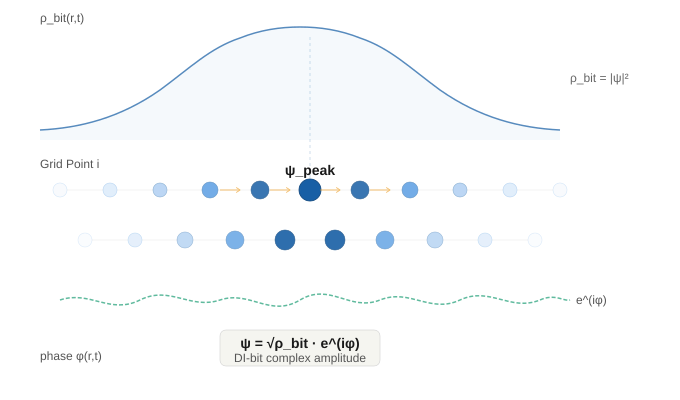
\includegraphics[width=0.90\textwidth]{qm2040a_fig1_gaussian_packet.pdf}
\caption{Gaussian DI-bit wave packet on the 600-cell lattice.
  Grid Points (circles) are coloured by local DI-bit density
  $\rho_{\rm bit}$ (dark blue $=$ high, pale blue $=$ low),
  following the Gaussian envelope $\rho_{\rm bit}(r,0) \propto
  e^{-r^2/2\sigma^2}$ shown as the upper curve.
  Amber arrows indicate the direction of coherent DI-bit flow.
  The lower dashed curve shows the phase oscillation $e^{i\phi}$.
  The total DI-bit complex amplitude $\psi = \sqrt{\rho_{\rm bit}}\,e^{i\phi}$
  encodes both density and phase at each Grid Point.}
\label{fig:gaussian}
\end{figure}

%=====================================================================
\section{Lattice Hopping Hamiltonian}
%=====================================================================

Over one tick $\Delta t = \tP$ the amplitude at site $i$ evolves as
\begin{equation}
\psi_i(t+\Delta t) = \psi_i(t) - \frac{i\Delta t}{\hbar}
\sum_j H_{ij}\,\psi_j(t),
\label{eq:evolution}
\end{equation}
where
\begin{equation}
H_{ij} = \begin{cases}
-T & j \sim i \text{ (nearest neighbour)}, \\
+z\,T & j = i, \quad z = 12, \\
0 & \text{otherwise},
\end{cases}
\quad T = \frac{\hbar^2}{4m\,\Delta s^2}.
\label{eq:H}
\end{equation}

The factor $-i/\hbar$ is not postulated: it is the mathematical
translation of \emph{phase accumulation per hop}.  Classical diffusion
would replace $-i$ by $+D$ (real, positive); the imaginary unit is the
direct signature of phase-carrying DI bits.

\begin{remark}[Why $T = \hbar^2/(4m\Delta s^2)$, not $\hbar^2/(2m\Delta s^2)$]
The icosahedral 600-cell has $z=12$ nearest neighbours in 3D.
The graph Laplacian over all 12 neighbours yields
$(\mathcal{A}\psi)/\Delta s^2 \to 2\nabla^2\psi$ (Appendix~A).
The factor 2 is absorbed into the denominator of $T$: with
$T = \hbar^2/(4m\Delta s^2)$ and the factor of 2 from the Laplacian,
$-T \times 2\Delta s^2\nabla^2\psi = -\hbar^2\nabla^2\psi/(2m)$,
which is the correct kinetic operator.
Using $T = \hbar^2/(2m\Delta s^2)$ would give $-\hbar^2\nabla^2\psi/m$
(wrong by a factor of 2).
\end{remark}

%=====================================================================
\section{Continuum Limit: The Schr\"{o}dinger Equation}
%=====================================================================

\begin{theorem}[Schr\"{o}dinger equation from DI-bit hopping]
\label{thm:schrodinger}
In the continuum limit $\Delta s \to 0$ (holding $T\Delta s^2
= \hbar^2/(4m)$ fixed), the discrete hopping equation~\eqref{eq:evolution}
becomes
\begin{equation}
i\hbar\,\frac{\partial\psi}{\partial t}
= -\frac{\hbar^2}{2m}\nabla^2\psi + V(\mathbf{r})\psi,
\label{eq:Schrodinger}
\end{equation}
where $V(\mathbf{r}) = -k_{\rm PSR}\,\Delta|\SSV(\mathbf{r})|$ is
the external potential sourced by the Space Stress Vector field.
\end{theorem}

\begin{proof}
From the 600-cell graph Laplacian (Appendix~A):
$\sum_{j\sim i}(\psi_j - \psi_i) = 2\Delta s^2\nabla^2\psi
+ O(\Delta s^4)$.  Substituting into~\eqref{eq:evolution}:
\begin{equation}
i\hbar\,\frac{\psi_i(t+\Delta t) - \psi_i(t)}{\Delta t}
= -T\bigl(\mathcal{A}\psi\bigr)_i + V_i\psi_i
= -\frac{\hbar^2}{4m\Delta s^2}\cdot 2\Delta s^2\nabla^2\psi + V\psi
= -\frac{\hbar^2}{2m}\nabla^2\psi + V\psi.
\end{equation}
Taking $\Delta t \to 0$ gives~\eqref{eq:Schrodinger}. \qed
\end{proof}

\begin{figure}[H]
\centering
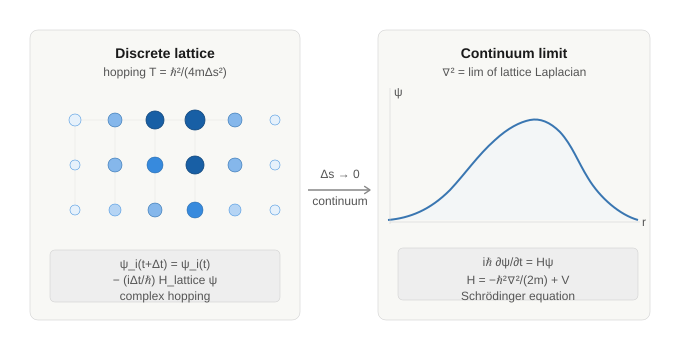
\includegraphics[width=0.90\textwidth]{qm2040a_fig2_discrete_continuum.pdf}
\caption{Discrete-to-continuum transition.
  \textit{Left:} Discrete 600-cell lattice with DI-bit amplitudes
  (colour $=$ density, arrows $=$ hopping direction).  The master equation
  governs complex amplitude hopping at each tick.
  \textit{Right:} Smooth wavefunction $|\psi(r,t)|^2$ from the continuum
  limit.  The lattice Laplacian $(\mathcal{A}\psi)/\Delta s^2 \to 2\nabla^2\psi$
  connects the two descriptions via Theorem~\ref{thm:schrodinger}.}
\label{fig:discrete_continuum}
\end{figure}

%=====================================================================
\section{Madelung Decomposition and Quantum Pressure}
%=====================================================================

\begin{proposition}[Madelung transformation]
Writing $\psi = \sqrt{\rho}\,e^{iS/\hbar}$ and substituting
into~\eqref{eq:Schrodinger} gives the real pair:
\begin{align}
\frac{\partial\rho}{\partial t}
+ \nabla\cdot\!\left(\rho\,\frac{\nabla S}{m}\right) &= 0,
\label{eq:continuity}\\
\frac{\partial S}{\partial t}
+ \frac{(\nabla S)^2}{2m} + V - Q &= 0,
\label{eq:HJ}
\end{align}
where the quantum pressure is
$Q = -\hbar^2\nabla^2\!\sqrt{\rho}/(2m\sqrt{\rho})$.
\end{proposition}

Equation~\eqref{eq:continuity} is DI-bit number conservation, enforced
by the Nexus.  The quantum pressure $Q$ in~\eqref{eq:HJ} is the
geometric interference effect of phase-carrying DI bits arriving from
regions of different density; it is not postulated but emerges
automatically from the complex hopping.

%=====================================================================
\section{Predictions}
%=====================================================================

At all laboratory wavelengths $\lambda \gg \lP$, lattice corrections
to quantum dynamics are of order $(\lP/\lambda)^2 \lesssim 10^{-58}$
(optical) and unobservable.  In the energy spectrum of bound states:
\begin{equation}
E_n^{\rm CPP} = E_n^{\rm QM}\bigl[1 + c_n(\lP/\lambda_n)^2
+ O(\lP/\lambda_n)^4\bigr].
\end{equation}
These corrections are in principle falsifiable: a measurement of
atomic energy levels at precision $\gg 10^{-50}$ relative accuracy
would probe the lattice structure.

%=====================================================================
\section{Conclusion}
%=====================================================================

The Schr\"{o}dinger equation emerges in CPP from complex phase-carrying
DI-bit hopping on the 600-cell lattice.  The derivation uses no
diffusion step; the imaginary unit arises from phase accumulation per
hop.  The quantum pressure term is automatic, not postulated.  The
key corrected result: $T = \hbar^2/(4m\Delta s^2)$, not
$\hbar^2/(2m\Delta s^2)$, to account for the factor of 2 from the
12-neighbour graph Laplacian of the 600-cell.

%=====================================================================
\appendix
\section{Graph Laplacian of the 600-Cell in 3D}
\label{app:laplacian}
%=====================================================================

The 600-cell has coordination number $z=12$ in 3D ($d=3$).
For a smooth function $\psi(\mathbf{r})$ and vertex $i$ at $\mathbf{r}_i$:
\begin{equation}
\sum_{j\sim i}(\psi_j - \psi_i)
= \tfrac{1}{2}\,\frac{z\,\Delta s^2}{d}\,\nabla^2\psi + O(\Delta s^4)
= 2\,\Delta s^2\,\nabla^2\psi + O(\Delta s^4).
\end{equation}
The first step uses icosahedral symmetry ($\sum_j\Delta\mathbf{r}_{ij}=0$,
$\sum_j(\Delta\mathbf{r}_{ij})^2 = z\Delta s^2\mathbf{1}/d$);
the numerical value $z/(2d) = 12/6 = 2$ is a property of the 600-cell.

%=====================================================================
\ibliographystyle{plainnat}
\ibliography{cpp_qm_series}


\section*{Acknowledgements}
The CPP programme is registered at OSF (DOI:~\url{https://doi.org/10.17605/OSF.IO/JXE8D}) and maintained at GitHub (\url{https://github.com/Hyperphysics-Institute/CPP}).

\bibliographystyle{plainnat}
\bibliography{cpp_qm_series}

\end{document}
